\section{Versuchsaufbau/-durchführung}
Der verwendete Versuchsaufbau ist in Abbildung \ref{fig: aufbau} dargestellt.
\begin{figure}
  \centering
  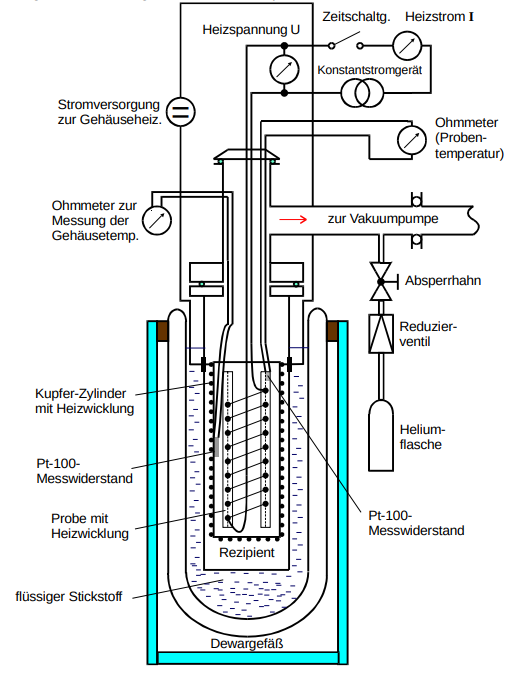
\includegraphics[width = 0.65\textwidth]{./content/images/aufbau.png}
  \caption{Schematische Darstellung des experimentellen Aufbaus des Versuchs V46  \cite{anleitungV47}.}
  \label{fig: aufbau}
\end{figure}
Zunächst wird der in der Darstellung \ref{fig: aufbau} abgebildete Rezipient
mit Hilfe einer Drehschieberpumpe evakuiert. Anschließend wird in den Rezipient
Helium eingefüllt. Mit dem Helium soll verhindert werden, das sich die Restluft
(insbesondre der Stickstoff) im Rezipient verflüssigt oder das sich Wasserkristalle
ausbilden. Die in einem Dewaregefäß befindliche Rezipient wird nun mit flüssigen
Stickstoff auf eine Temperatur von ca. $\SI{80}{\kelvin}$ abgekühlt. Ist die
Zieltemperatur erreicht wird das Helium mit der Drehschieberpumpe abgepumpt und
ein Vakuum erzeugt. Nun wird soll die sich in einem Kupferzylinde befindliche
Kupferprobe langsam erhizt werden. Hierbei wurde wahrscheinlich Kufper als Material
für den Zylinder gewählt, damit dieser den selben Wärmestrahlungskoeffizient besitzt
wie Kufper. Wie in Abbildung \ref{fig: aufbau} dargestellt, werden für das erhitzen
Heizwickeln verwendet. Die Temperatur der Heizwickeln können über zwei
Stromquellen gesteuert werden. Eine Temperaturmessung erfolgt über zwei
Pt-100 Messwiderstände. Bei der Erwärmung der Probe ist darauf zu achten, dass
die Temperaturerhöhung $\Delta T$ lediglich durch die elektrische Energie $E$
der Heiwicklung gegeben ist. Aus diesem Grund wird der Rezipient in einem
Vakuum erwärmt - dies verhindert Energieverluste durch Konvektion, Wärmestrahlung und
Wärmeleitung. Zusätzlich muss mit Hilfe der beiden Stromquellen sichergestellt
werden, dass die Probe und der Kupferzylinder zu jedem Zeitpunkt die annähernd
selbe Temperatur aufweisen. Wie schon in dem Kapitel $\ref{sec:theorie}$ erwähnt
ist es experimentel leichter zu realisieren $C\ua{p}$ zu messen.
Hierzu wird der Temperaturanstieg $\Delta T$ sogewählt, das er bei
etwa $7-\SI{11}{\degreeCelsius}$ pro $\SI{5}{\minute}$ liegt. Nach dieser Zeit werden die
Widerstände der beiden Pt-100, die Spannung und Stromstärke der Probenheizung notiert.
Mit diesen Messdaten, der Probenmasse und dem Molekulargewicht lässt sich $C\ua{p}$
berechnen.  
